% ---------
%  Compile with "pdflatex hw1".
% --------
%!TEX TS-program = pdflatex
%!TEX encoding = UTF-8 Unicode

% Template borrowed from Jeff Erickson.

\documentclass[11pt]{article}
\usepackage{jeffe,handout,graphicx}
\usepackage[utf8]{inputenc}		% Allow some non-ASCII Unicode in source
\usepackage{xcolor}
\usepackage{mdframed}
\usepackage{arydshln}
\usepackage{svg}
\usepackage{cite}
\usepackage{cleveref}

% =========================================================
%   Define common stuff for solution headers
% =========================================================
\Class{CS 7301.003}
\Semester{Fall 2020}
\Authors{2}
\AuthorOne{Dongpeng Liu}{dxl200000}
\AuthorTwo{Jiashuai Lu}{jxl173630}
%\Section{}

% =========================================================
\begin{document}
\HomeworkHeader{2}{1}% homework number, problem number
% ---------------------------------------------------------
Describe an algorithm to determine whether two given polygonal arcs \(\alpha\) and \(\beta\) are relatively homotopic. You should attempt to justify your algorithm’s correctness, but you do not need to give a formal proof.

\begin{solution}\(\)\par

  \begin{algo}
    \textul{\(\textsc{TestRelativeHomotopy}(\alpha, \beta, \mathscr{P})\):}\+
    \\  Compute a frugal triangulation \(\Delta\) for \(R^2\backslash S\) where \(S\) are set of sentinels as \(P_1,\dots,P_h\).
    \\  Let \(C_0\) be the set of edges in \(\Delta\) that has one end point at the outer boundary of \(R^2\backslash S\). Sort \(C_0\)
    \\  in clockwise order w.r.t the sub-triangulation consists of all edges between \(S\).
    \\  Let \(Y\) be the label sequence for edges in \(C_0\). Let \(Y^{-1}\) be its reversal.
    \\
    \\  Compute reduced crossing sequence \(X_\Delta(\alpha)\) and \(X_\Delta(\beta)\).
    \\  While \(X_\Delta(\alpha)\) or \(X_\Delta(\beta)\) starts or ends with a substring \(X'\) of length \(|Y|\) s.t. \(X'\) is a substring of \(Y\cdot Y\) or
    \\  \(Y^{-1}\cdot Y^{-1}\)\+
    \\    Cut off \(X'\) from \(X_\Delta(\alpha)\) or \(X_\Delta(\beta)\).\-
    \\  Let \(\alpha_0,\alpha_1\) and \(\beta_0,\beta_1\) be the start and end of \(\alpha\) and \(\beta\), respectively.
    \\  Let \(\pi_c/\pi_{cc}\) be the path from \(\beta_0\) to \(\alpha_0\) through \(P_0\) clockwisely/counter-clockwisely.
    \\  Let \(\delta_c/\delta_{cc}\) be the path from \(\alpha_1\) to \(\beta_1\) through \(P_0\) clockwisely/counter-clockwisely.
    \\  Compute crossing sequences \(X_\Delta(\pi_c),X_\Delta(\pi_{cc}), X_\Delta(\delta_c), X_\Delta(\delta_{cc})\).
    \\  for \(\pi \in {\pi_c,\pi_{cc}}\)\+
    \\      for \(\delta\in {\delta_c,\delta_{cc}}\)\+
    \\          if reduced sequence of \(X_\Delta(\pi)\cdot X_\Delta(\alpha)\cdot X_\Delta(\delta)\) equals to \(X_\Delta(\beta)\)\+
    \\              Return \(\alpha\) and \(\beta\) are relative homotopy.\-\-\-
    \\  Return \(\alpha\) and \(\beta\) are not relative homotopy.
  \end{algo}
\end{solution}

\HomeworkHeader{2}{2}% homework number, problem number
Prove that for some constants \(\Delta\), \(\Delta_*\), and \(c\), any simple \(n\)-vertex plane graph \(G\) can be modified by inserting subgraphs or expanding vertices into a new simple planar graph \(\Tilde{G}\) with \(cn\) vertices, such that each vertex has degree at most \(\Delta\) and each face has degree at most \(\Delta_*\). More simply: Argue that without loss of generality, simple plane graphs have bounded vertex degrees and bounded face degrees. You do not need to give exact values for these constants, but do argue that they exist.

\textit{[Hint: Start by expanding all high degree vertices. Then, for each large face, subdivide it
by inserting a single smaller face (not necessarily of constant size) surrounded by a constant
number of faces of constant size, and recurse.]}

\begin{solution}
  We use \(d_v\) to denote degree of vertex \(v\) and \(D_f\) to denote degree of face \(f\). W.l.o.g. we assume \(\Delta\ge 6\) and \(\Delta^*\ge 5\).

  \noindent First we expand every vertex with degree \(>\frac{\Delta}{2}\) as follows:\vspace{-5pt}
  \begin{enumerate}[(V.1)]\itemsep0pt
  \item Split \(v\) to \(v_0\) and \(v_1\) and add an edge between \(v_0\) and \(v_1\) such that \(\frac{\Delta}{2}-2\) edges incident to \(v\) are incident to \(v_0\) and other \(d_v-\frac{\Delta}{2}+2\) edges incident to \(v\) are incident to \(v_1\) without breaking the planarity.
  \item If \(d_{v_1}>\frac{\Delta}{2}\), let \(v\from v_1\), repeat step \((1)\). Otherwise, we finished expanding \(v\).
  \end{enumerate}

  \noindent Then we subdivide every face \(f\) with degree \(>\Delta^*\) as follows:\vspace{-5pt}
  \begin{enumerate}[(F.1)]\itemsep0pt
  \item We add a face \(f^*\) of degree \(\ceil{\frac{D_f}{\Delta^*-3}}\) inside \(f\) and disjoint with \(f\).
  \item By connecting each vertex of \(f^*\) to a unique vertex of \(f\), we can subdivide \(f\backslash f^*\) into \(\ceil{\frac{D_f}{\Delta^*-3}}\) faces. Furthermore, each of those faces has degree at most \(\Delta^*\), the degree of vertex of \(f\) increase by at most \(1\), the degree of vertex of \(f^*\) is at most \(3\le \frac{\Delta}{2}\). See Figure~\ref{fig:degree1} as an example.
  \item If \(D_{f^*}>\Delta^*\), let \(f\from f^*\), repeat from step \(1\). Otherwise, we move to next \(f\) with \(D_f>\Delta^*\).
  \end{enumerate}\vspace{-3pt}
  \begin{figure}[h]
  \centering
  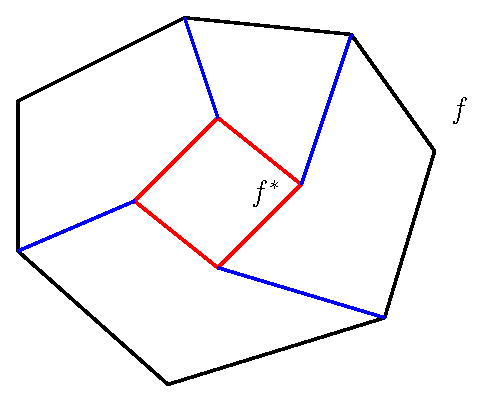
\includegraphics[scale=0.5]{fig/prob2-1.eps}
  \caption{An example of \(\Delta^*=5\)}
  \label{fig:degree1}
\end{figure}

Let \(\Tilde{G}\) be the resulting plane graph. We show that \(\Tilde{G}\) has every vertex with degree at most \(\Delta\) and every face with degree at most \(\Delta^*\), and the number of vertices in \(\Tilde{G}\) is at most \(cn\).

Notice that for every vertex \(v\in G\) with \(d_v>\frac{\Delta}{2}\), step \(1\) will be repeated by at most \(\frac{d_v}{\Delta/2-2}\) times. Every repetition increase the number of vertices by one. So in the vertex expanding phase, the number of vertices increased by at most \(O(\frac{\sum_{v}d_v)}{\Delta/2-2})\le O(\sum_{v}d_v)\le O(n)\). Moreover, now every vertex in the graph has degree \(\le \frac{\Delta}{2}.\)

In the face subdividing phase, for every face \(f\), step \(1\) will be run at most \(\log_{\Delta^*-3}D_f\) times.
The degree of \(f\) is decreasing exponentially by a factor \(\Delta^*-3\ge 2\).
So the total number of vertices increases by at most \(2D_f\).
Summing all faces together, at most \(O(\sum_fD_f)\le O(n)\) vertices are added in this phase.

Recall that every face in \(f\backslash f^*\) has degree at most \(\Delta^*\) and we will not touch them at any other time.
The degree of every vertex of \(f\) could be increased by at most \(1\) when we process \(f\).
Therefore, the degree increase of every vertex \(d_v\) during the subdividing phase is at most the number of faces sharing \(v\) (\(\le d_v\)).
Since \(d_v\le \frac{\Delta}{2}, \forall v\) before subdividing phase, those vertices will have degrees at most \(\Delta\) in \(\Tilde{G}\).

In step \(\mathsc{F}.2\), every vertex of \(f^*\) has degree \(3\le \frac{\Delta}{2}\), the degree of any of those vertices could be possibly increased by at most one during the following recursions on \(f^*\). Therefore, every vertex in \(\Tilde{G}\) has degree at most \(\Delta\) and every face has degree at most \(\Delta^*\) while the number of vertices in \(\Tilde{G}\) is at most \(O(n)\).

So we showed for some constants \(\Delta\ge 6, \Delta^*\ge 5\) and \(c\), we can modify any simple \(n\)-vertex plane graph \(G\) into a simple \(cn\)-vertex plane graph \(\Tilde{G}\) with vertex degree at most \(\Delta\) and face degree at most \(\Delta^*\).
\end{solution}

\HomeworkHeader{2}{3}% homework number, problem number
\begin{enumerate}[(a)]
\item Prove that a directed plane graph \(G\) is acyclic if and only if the dual graph \(G^*\) is strongly connected.
  \begin{solution}
    First we prove if \(G\) is acyclic, then \(G^*\) is strongly connected.

    Assume by contradiction we have a graph \(G\) is acyclic but its dual graph \(G^*\) is not strongly connected.
    Then there exists at least a pair of dual vertices \(f^*,g^*\) in \(G^*\) such that there is no directed path from \(f^*\) to \(g^*\) in \(G^*\). So there exists a cut \((S^*,G^*\backslash S^*)\) such that \(f^*\in S^*, g^*\in G^*\backslash S^*\) and every dual edge \(e^*\) in this cut has tail \(\mathrm{left}(e)^*\) in \(G^*\backslash S^*\) and head \(\mathrm{right}(e)^*\) in \(S^*\). Which means in the corresponding primal cycle of this cut in \(G\), every edge \(e\) has its right shore in \(S\). This cycle is a clockwise cycle w.r.t. \(S\). A contradiction. So \(G^*\) is strongly connected.

    Then we show if \(G^*\) is strongly connected, then \(G\) is acyclic. Similarly as the arguments above, we could see that if \(G^*\) is strongly connected, then there does not exist directed cut in \(G^*\). So there is also no directed cycle in \(G\).

  \end{solution}
\item Call an edge of a directed graph \(G\) internal if its endpoints lie in the same strong component of \(G\) and external otherwise. Prove that an edge \(e\) in a directed plane graph \(G\) is internal if and only if the corresponding dual edge \(e^*\) of the dual graph \(G^*\) is external.
  \begin{solution}
    We first show if \(e\) in \(G\) is internal then the dual edge \(e^*\) in \(G^*\) is external.
    Let \(S\) be the strong component of \(G\) where two endpoints of \(e\) lies in. Then we know \(S^*\) is acyclic from subproblem \((\mathrm{a})\).
    Let \(f^*,g^*\) be the tail and head of \(e^*\). Then there is no path from \(g^*\) to \(f^*\) in \(S^*\). So \(f^*\) and \(g^*\) not lie in the same strong component.

    If the dual edge \(e^*\) is external, then \(f^*\) and \(g^*\) lie in different strong components of \(G^*\), and there exists no paths in \(G^*\) from \(g^*\) to \(f^*\). This implies that there exists a directed dual cut in \(G^*\) separate \(f^*, g^*\) into two partitions and \(e^*\) must be in this dual cut. Correspondingly, \(e\) is in a directed cycle dual to this directed cut in \(G\). Since a directed cycle itself is strong connected, two endpoints of edge \(e\) must be in the same strong component of \(G\). Thus, \(e\) is internal in \(G\).

  \end{solution}

\end{enumerate}
\end{document}

%%% Local Variables:
%%% mode: latex
%%% TeX-master: t
%%% End:
